
\begin{question}
In a very large population, 88.1\% are special. When a random sample of
size 4200 is taken, what is the chance that the sample proportion of
special individuals is farther than \(\pm\) 0.5 percentage points from
88.1\%?
\end{question}

\begin{solution}
Determine the standard error.
\[SE = \sqrt{\frac{p(1-p)}{n}} = \sqrt{\frac{0.881(1-0.881)}{4200}} = 0.005 \]
Determine the upper and lower bounds on \(\hat{p}\).
\[\hat{p}_{\text{lower}} = 0.881-0.005 = 0.876 \]
\[\hat{p}_{\text{upper}} = 0.881+0.005 = 0.886 \] Determine the \(z\)
scores. For simplicity, we ignore the continuity correction.
\[z_{\text{lower}} = \frac{\hat{p}_{\text{lower}}-p}{SE} = \frac{0.876-0.881}{0.005} = 
\frac{-0.005}{0.005} = -1 \]
\[z_{\text{upper}} = \frac{\hat{p}_{\text{upper}}-p}{SE} = \frac{0.886-0.881}{0.005} = \frac{0.005}{0.005} = 1 \]
We are looking for a two-tail area (``farther than \(\pm\) 0.5
percentage points from 88.1\%'').

\begin{figure}[htbp]
\centering
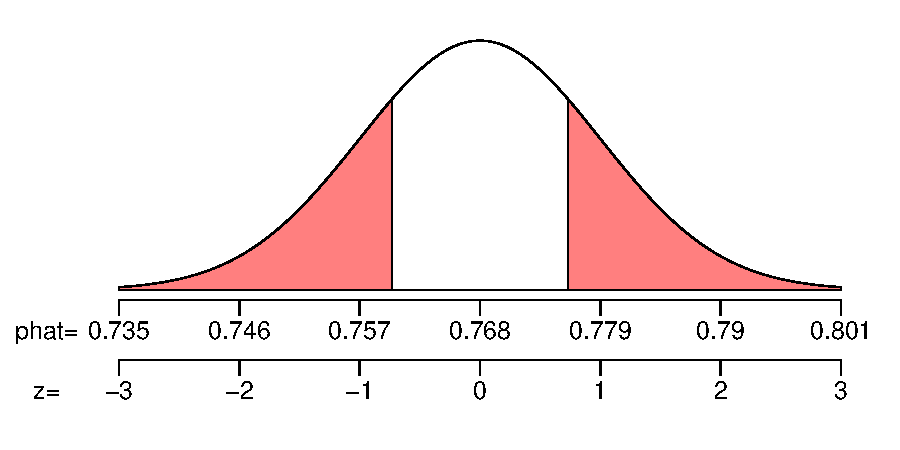
\includegraphics{phat_sampling_outer-1.pdf}
\caption{}
\end{figure}

To determine that central area, we use the z table.
\[\text{Pr}\left(|\hat{P}-0.881| > 0.005\right) ~~=~~ \text{Pr}\left(|Z| > 1\right) ~~=~~ 2\cdot\Phi(-1) ~~=~~ 0.3173 \]
Thus, we conclude there is a 31.7\% chance that the sample proportion is
farther than \(\pm\) 0.5 percentage points from 88.1\%.
\end{solution}

